\begin{figure}
    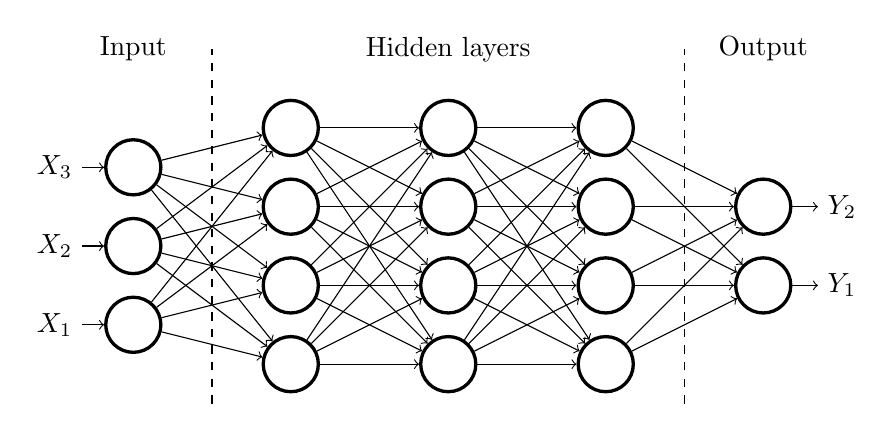
\begin{tikzpicture}[
        roundnode/.style={circle, draw=black, very thick, minimum size=7mm}
    ]
        \pgfmathsetmacro{\nin}{3}
        \pgfmathsetmacro{\nhl}{3}
        \pgfmathsetmacro{\nhn}{4}

        \foreach \i in {1,...,\nin}
        {
            \node at (-1, \i) (\i) {$X_\i$};
            \node[roundnode] at (0, \i) (i\i) {};
            \draw[->] (\i) -> (i\i);
        }

        \foreach \i in {1,...,\nhl}
        {
            \pgfmathsetmacro{\yshift}{(\nin - \nhl)/2}
            \foreach \j in {1,...,\nhn}
            {
                \node[roundnode] at (2*\i, -0.5+\j) (h\i\j) {};
            }
        }

        \foreach \i in {1,...,\nin}
        {
            \foreach \j in {1,...,\nhn}
            {
                \draw[->] (i\i) -- (h1\j);
            }
        }

        \foreach \i in {1,...,2}
        {
            \pgfmathtruncatemacro{\x}{\i +1};
            \foreach \j in {1,...,\nhn}
            {
                \foreach \k in {1,...,\nhn}
                {
                    \draw[->] (h\i\j) -- (h\x\k);
                }
            }
        }

        \foreach \i in {1,...,2}
        {
            \node[roundnode] at (8, 0.5+\i) (o\i) {};
            \foreach \j in {1,...,4}
            {
                \draw[->] (h3\j) -- (o\i);
            }
            \node at (9, 0.5+\i) (y\i) {$Y_\i$};
            \draw[->] (o\i) -- (y\i);
        }

        \draw [dashed] (1, 0) -- (1, 4.5);
        \draw [dashed] (7, 0) -- (7, 4.5);
        \node at (0, 4.5) {Input};
        \node at (4, 4.5) {Hidden layers};
        \node at (8, 4.5) {Output};
    \end{tikzpicture}
\end{figure}
